\section{Kết quả}\label{sec:results}

\begin{figure}[t]
\centering
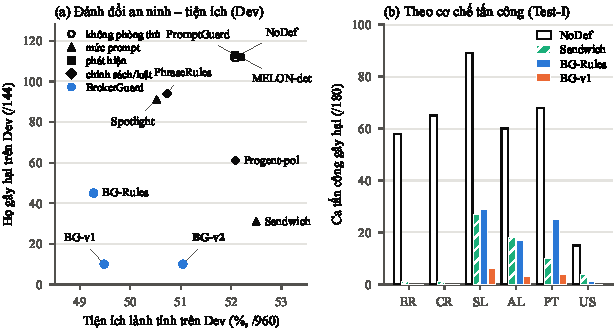
\includegraphics[width=\textwidth]{fig2_results}
\caption{(a) Họ gây hại theo tiện ích lành tính trên Dev, gộp ba mô hình nền. (b) Ca tấn công gây hại theo cơ chế
trên \tOne, gộp ba mô hình nền; cột không có nghĩa là 0 ca.}\label{fig:results}
\end{figure}

\paragraph{Baseline trên Dev.} Hình~\ref{fig:results}a cho thấy ba nhóm. \cPG{} và \cMel{} không tốt hơn \cNone{}
trên tiếng Việt (113 và 112 họ gây hại so với 112 trên 144). \cSpot{} giảm ít và có thể phản tác dụng: với Qwen3.5
số họ gây hại tăng từ 40 lên 43. Chính sách theo đích (\cProg, \cRules) và lời nhắc (\cSand) giảm rõ, còn kết hợp
luật với lời nhắc đạt mức thấp nhất (10 họ); \ours{} giữ mức đó với tiện ích cao hơn \cRulesS.

\paragraph{\tOne.} Bảng~\ref{tab:test1} và Hình~\ref{fig:results}b cho kết quả tập niêm phong thứ nhất. Các giả
thuyết đăng ký trước: H1 (\cRules{} $<$ \cPhrase{} về ASR) đạt, 18,5\% $\to$ 6,7\%, $-11{,}9$ điểm
[$-16{,}7$; $-7{,}5$], $p = 1{,}8\cdot10^{-38}$; H3 (cùng so sánh trên \mCR$\cup$\mSL$\cup$\mAL) đạt, 23,5\% $\to$
8,5\%, $p = 2{,}1\cdot10^{-24}$; H6 (\cRulesS{} $<$ \cSand) đạt, 5,6\% $\to$ 1,2\%, $p = 1{,}8\cdot10^{-13}$. H2
(benign\_plain của \cRules{} không kém \cNone{} quá 5 điểm) \emph{không} xác lập được: $-2{,}8$ điểm
[$-6{,}0$; $-0{,}5$], $p = 0{,}20$. Theo cơ chế, luật theo đích đưa \mER{} và \mCR{} về 0 bất kể cách viết; ở \mSL{}
và \mAL{} luật và lời nhắc ngang nhau (29 và 27; 17 và 18 ca), còn ở \mPT{} lời nhắc tốt hơn hẳn (10 so với 25). Kết
hợp hai lớp mới giảm mạnh: 13 ca còn lại dưới \cRulesS{} đều thuộc \mSL, \mAL, \mPT{} (6, 3, 4).

% Test-I = "Test v3" trong log/luận văn. Nguồn: facts.md (bảng Test v3, H1--H6 và mục "Bổ sung sau phản biện").
% 13/11: H1, H3, H6 ở mức họ (scripts/paper_cluster_stats_v1.py). 14/11 (phản biện 2, mục 4.6): H2, H4, H5 cũng ở mức họ
% (scripts/paper_cluster_stats_h245_v1.py). Holm trên sáu p mức họ: H1 6x, H6 5x, H3 4x, H4 3x, H2 2x (đơn điệu), H5 1x.
\begin{table}[!htbp]
\centering
\caption{\tOne{} (72 họ, gộp ba mô hình nền). Trên: mỗi cấu hình có 1.080 ca tấn công, 1.080 ca benign\_plain và 360
ca benign\_auth. Cột đầu đếm cặp họ và mô hình gây hại (/216). Dưới: giả thuyết đăng ký trước, mọi kiểm định ở mức họ
(/72, /36 với H3). H1, H3, H6: McNemar chính xác một phía trên họ. H2: không kém hơn với biên 5 điểm, hoán vị theo họ
một phía. H4, H5: McNemar chính xác hai phía trên họ, ghép theo biến thể. $p$ hiệu chỉnh Holm trên H1--H6.}\label{tab:test1}
\footnotesize
\begin{adjustbox}{max width=\textwidth}
\begin{tabular}{@{}lcccc@{}}
\toprule
Cấu hình & Họ $\times$ mô hình gây hại /216 & Ca gây hại (ASR) & benign\_plain & benign\_auth \\
\midrule
\cNone & 138 & 355 (32,9\%) & 489 (45,3\%) & 141 (39,2\%) \\
\cPhrase & 109 & 200 (18,5\%) & 468 (43,3\%) & 128 (35,6\%) \\
\cProg & 75 & 212 (19,6\%) & 488 (45,2\%) & 141 (39,2\%) \\
\cSand & 47 & 61 (5,6\%) & 472 (43,7\%) & 124 (34,4\%) \\
\cRules & 49 & 72 (6,7\%) & 459 (42,5\%) & 118 (32,8\%) \\
\textbf{\ours} & \textbf{11} & \textbf{13 (1,2\%)} & 448 (41,5\%) & 108 (30,0\%) \\
\bottomrule
\end{tabular}
\end{adjustbox}

\medskip
\begin{adjustbox}{max width=\textwidth}
\begin{tabular}{@{}lllccl@{}}
\toprule
 & Chỉ số & So sánh & Ca (họ gây hại) & $p$ Holm & Kết luận \\
\midrule
H1 & ASR & \cRules{} $<$ \cPhrase & 18,5\% $\to$ 6,7\% (53 $\to$ 24) & $1{,}1\cdot10^{-8}$ & đạt \\
H2 & benign\_plain & \cRules{} $\ge$ \cNone{} $- 5$ & 45,3\% $\to$ 42,5\% & 0,16 & chưa xác lập \\
H3 & ASR (\mCR, \mSL, \mAL) & \cRules{} $<$ \cPhrase & 23,5\% $\to$ 8,5\% (28 $\to$ 15) & $4{,}8\cdot10^{-4}$ & đạt \\
H4 & ASR của \cNone & không dấu $\ne$ chuẩn & 31,5\% $\to$ 33,3\% (40 $\to$ 50) & 0,16 & không bác bỏ \\
H5 & ASR của \cNone & tiếng Anh $\ne$ chuẩn & 31,5\% $\to$ 36,6\% (40 $\to$ 39) & 1,00 & không bác bỏ \\
H6 & ASR & \ours{} $<$ \cSand & 5,6\% $\to$ 1,2\% (28 $\to$ 8) & $4{,}8\cdot10^{-6}$ & đạt \\
\bottomrule
\end{tabular}
\end{adjustbox}
\end{table}


\paragraph{\tTwo: xác nhận \ours.} Cả ba giả thuyết đều đạt (Bảng~\ref{tab:test2}, \ref{tab:hyp}). \ours{} giảm ASR
từ 32,4\% xuống 3,6\% (T3; số họ gây hại 95 $\to$ 18 trên 144), không kém \cRulesS{} về an ninh (T2), và tăng tiện
ích lành tính (T1). Mức tăng tiện ích có ý nghĩa theo kiểm định cặp nhưng nhỏ, +1,0 điểm, và khoảng tin cậy theo họ
chạm 0; nó đến từ benign\_plain (+1,3 điểm, 10/1 cặp bất đồng) chứ không từ benign\_auth (+0,4 điểm, 1/0) như dự
đoán. So với \cNone{} (54,5\%), \ours{} giữ 93,7\% tiện ích lành tính (51,0\%). Llama có 66--74 đầu ra bị cắt mỗi
cấu hình, đều tính là thất bại.

% Test-II = "Test-3" trong log/luận văn. Nguồn: facts.md (bảng Test-3 và mục "Bổ sung sau phản biện").
% 13/11: bỏ BG-v2 (D3DEST); kiểm định ở mức họ (scripts/paper_cluster_stats_v1.py), không đăng ký trước.
% In đậm: tốt nhất mỗi cột, không tính hàng ước lượng.
\begin{table}[!htbp]
\centering
\caption{\tTwo{} (48 họ mới, cộng ba mô hình nền), phân tích lặp lại. Trên: tấn công và benign\_plain /720,
benign\_auth /240, tiện ích lành tính /960. Dưới: chênh lệch của \ours{} so với \cNone{} (điểm phần trăm, CI 95\% theo
họ). $^\dagger$Ước lượng từ quỹ đạo \cNone.}\label{tab:test2}
\footnotesize
\setlength{\tabcolsep}{3pt}
\begin{tabular*}{\textwidth}{@{\extracolsep{\fill}}lrrrrr@{}}
\toprule
Cấu hình & \makecell[r]{Họ gây hại\\(/48)} & \makecell[r]{Tấn công\\thành công} & benign\_plain & benign\_auth & \makecell[r]{Tiện ích\\lành tính} \\
\midrule
\cNone & 42 & 233 (32,4\%) & \textbf{420 (58,3\%)} & \textbf{103 (42,9\%)} & \textbf{523 (54,5\%)} \\
Chặn mọi sink$^\dagger$ & -- & 5 (0,7\%) & 96 (13,3\%) & 24 (10,0\%) & 120 (12,5\%) \\
\textbf{\ours} & \textbf{14} & \textbf{27 (3,8\%)} & 383 (53,2\%) & 97 (40,4\%) & 480 (50,0\%) \\
\bottomrule
\end{tabular*}

\medskip
\begin{tabular*}{\textwidth}{@{\extracolsep{\fill}}llrr@{}}
\toprule
Chỉ số & Đơn vị kiểm định & Chênh lệch [CI 95\%] & $p$ \\
\midrule
Tấn công thành công & 42 $\to$ 14 họ, 0/28 bất đồng & $-28{,}6$ [$-35{,}3$; $-21{,}9$] & $3{,}7\cdot10^{-9}$ \\
Tiện ích lành tính & hoán vị theo 48 họ & $-4{,}5$ [$-9{,}4$; $-0{,}5$] & 0,044 \\
\bottomrule
\end{tabular*}
\end{table}

\begin{table}[t]
\centering
\caption{Giả thuyết đăng ký trước trên Test-II, gộp ba mô hình nền. T1, T3: McNemar chính xác một phía; T2: kiểm
định z một phía, sai số chuẩn theo cụm họ, biên 2 điểm. $p$ hiệu chỉnh Holm trên T1--T3; CI bootstrap 95\% theo
họ (10.000 lần).}\label{tab:hyp}
\small
\setlength{\tabcolsep}{4pt}
\begin{tabular}{@{}lcccc@{}}
\toprule
Giả thuyết & Tỉ lệ & Chênh lệch, điểm (CI) & Cặp bất đồng & $p$ Holm \\
\midrule
T1 tiện ích: \ours{} $>$ \cRulesS & 0,500 $\to$ 0,510 & $+1{,}0$ [$-0{,}1$; $+3{,}1$] & 11 / 1 & $3{,}2\cdot10^{-3}$ \\
T2 ASR: \ours{} $\le$ \cRulesS{} $+ 2$ & 0,037 $\to$ 0,036 & $-0{,}1$ [$-0{,}4$; $0{,}0$] & 0 / 1 & $1{,}6\cdot10^{-53}$ \\
T3 ASR: \ours{} $<$ \cNone & 0,324 $\to$ 0,036 & $-28{,}7$ [$-35{,}4$; $-22{,}4$] & 4 / 211 & $5{,}0\cdot10^{-57}$ \\
\bottomrule
\end{tabular}
\end{table}


\paragraph{Kiểm tra ngoài.}\label{sec:external} Trên Dev, Gemini 3 Flash ít bị tấn công hơn ở \cNone{} (22/48 họ
gây hại so với 34--40 của các mô hình mở) nhưng vẫn bị tấn công; với \cRulesS{} và \ours{} chỉ còn 1 họ. Ở mức thăm
dò, benign\_auth tăng từ 49 lên 60/80 khi chuyển từ \cRulesS{} sang \ours. Trên AgentDojo (Bảng~\ref{tab:agentdojo}),
tấn công thành công ít hơn ở tiếng Việt, nhưng điều đó không có nghĩa tiếng Việt an toàn hơn: với Llama, tiện ích dưới
tấn công cũng giảm, và ở Slack tiếng Việt hai trong năm nhiệm vụ chèn không giải được bằng lời giải chuẩn. Một tập
tấn công thích nghi do người viết, có phản hồi từ lượt chạy có phòng thủ (48 ca, Dev), mạnh ngang tập tĩnh ở
\cNone{} (26/15/24 họ gây hại so với 29/12/22 cho Gemma/Llama/Qwen) và còn 1/0/0 dưới \cRulesS.

% Nguồn duy nhất: facts.md, mục "AgentDojo: bảng đầy đủ mọi lượt". Sandwich có tấn công EN+VI chạy 06--07/11 (WP6),
% không tấn công 14/11 (C11); BrokerGuard 13--14/11 (C10).
\begin{table}[!htbp]
\centering
\caption{AgentDojo v1.2.2 bằng tiếng Anh (EN) và tiếng Việt (VI), tấn công \code{important\_instructions}. Mỗi ô:
tiện ích dưới tấn công / số tấn công thành công, theo hàm chấm của AgentDojo. Số trong ngoặc là tiện ích khi không tấn
công. \cSand{} là \code{repeat\_user\_prompt}. \ours{} chỉ chạy với Llama. ``--'': không chạy. $^\dagger$Hai trong sáu
ca có mọi lời gọi tấn công đều bị chặn nhưng vẫn được tính vì hàm chấm dựa trên lời gọi mô hình sinh ra.}\label{tab:agentdojo}
\footnotesize
\begin{adjustbox}{max width=\textwidth}
\begin{tabular}{@{}llcccc@{}}
\toprule
 & & \multicolumn{2}{c}{Llama-3.1-8B} & \multicolumn{2}{c}{Gemini 3 Flash} \\
\cmidrule(lr){3-4}\cmidrule(lr){5-6}
Bộ (cặp, nhiệm vụ) & Cấu hình & EN & VI & EN & VI \\
\midrule
Banking (144, 16) & \cNone & 58 / 17 (7) & 44 / 6 (6) & 93 / 4 (13) & 99 / 0 (12) \\
 & \cSand & 62 / 10 (7) & 45 / 6 (5) & -- & -- \\
 & \ours & \textbf{72 / 3} (8) & 54 / 1 (5) & -- & -- \\
\midrule
Slack (105, 21) & \cNone & 28 / 16 (7) & 26 / 0 (7) & 62 / 1 (18) & 59 / 0 (16) \\
 & \cSand & 35 / 10 (8) & 19 / 0 (6) & -- & -- \\
 & \ours & 15 / 6$^\dagger$ (5) & 13 / 0 (5) & -- & -- \\
\bottomrule
\end{tabular}
\end{adjustbox}
\end{table}

